\documentclass{classrep}
\usepackage[utf8]{inputenc}
\usepackage{color}
\usepackage{amsmath}
\usepackage{dirtytalk}
\usepackage{latexsym}
\usepackage{multirow}
\usepackage{graphicx}
\usepackage{float}

\studycycle{Informatyka, studia STACJONARNE, I st.}
\coursesemester{VI}

\coursename{Komputerowe systemy rozpoznawania}
\courseyear{2020/2021}

\courseteacher{prof. dr hab. inż. Adam Niewiadomski}
\coursegroup{poniedziałek, 12:00}

\author{
  \studentinfo{Hubert Gawłowski}{224298} \and
  \studentinfo{Kamil Kiszko-Zgierski}{224328} }

\title{Projekt 2.  Podsumowania lingwistyczne relacyjnych baz danych}

\begin{document}
\maketitle

Opis projektu ma formę artykułu naukowego lub raportu z zadania
badawczego/doświadczalnego/obliczeniowego (wg indywidualnych potrzeb związanych np. z
pracą inżynierską/naukową/zawodową). \\
\indent {\bf Wybrane sekcje (rozdziały sprawozdania) są uzupełniane wg wymagań w
opisie Projektu 2. i Harmonogramie Zajęć na WIKAMP KSR jako efekty zadań w~poszczególnych tygodniach}. 

\section{Cel}
Celem zadania jest zaimplementowanie lingwistycznej agregacji, tj. przedstawienie danych liczbowych za pomocą sformułowań w języku pozornie naturalnym. Owa implementacja zostanie wykonana w technologii Java z graficznym interfejsem użytkownika oraz z wykorzystaniem systemu zarządania bazą danych o nazwie MySql, a badania zostaną przeprowadzone w oparciu o bazę danych zawierającą statystyki zawodników ligi koszykówki NBA od sezonu 1996/1997 do 2019/2020.
\cite{nba_data}.  \\


\section{Charakterystyka podsumowywanej bazy danych}

Jako bazę danych w zadaniu wykorzystaliśmy bazę danych dotyczącą informacji o zawodnikach NBA (najbrdziej prestiżowej lidze koszykarskiej na świecie) z lat 1996 - 2019. Cała baza danych składa się z 22 kolumn zawierających informacje o danych zawodnika oraz jego statystykach różnego rodzaju. Baza danych ma charakter pliku csv i zawiera 11144 rekordy. Spośród kolumn wybraliśmy te, które zawierają wartości, naszym zdaniem, najlepiej nadające się do rozmycia. Atrybuty do rozmycia dobraliśmy tak, aby zgadzały się z definicją zmiennej lingwistycznej, która prezentuje się następująco \cite{niewiadomski19}: 
\begin{equation}
    L=<\mathcal{L}, H(L), X, G, K>
    \label{eqn_zmienna_lingwistyczna}
\end{equation}
gdzie: \newline $\mathcal{L}$ jest nazwą zmiennej lingwistycznej L, \newline H lub H(L) jest zbiorem terminów lingwistycznych $l_1, l_2, ..., l_N, N \in \mathbf{N}$, które są wartościami L, \newline $X$ jest przestrzenią rozważań, w której określa się zbiory rozmyte $S_1, S_2,..., S_N, N \in \mathbf{N}$, reprezentujące odpowiednio terminy $l_1, l_2, ..., l_N$, \newline $G$ jest regułą gramatyczną, która generuje terminy w zbiorze $H(L)$, \newline $K$ jest regułą semantyczną, która przyporządkowuje terminom $l_i$ zbiory rozmyte $S_i$ 2 $X$, czyli $K : l_i \rightarrow S_i, S_i = \{<x,\mu_{S_i}(x)> : x \in X \}, i = 1,2,...,N$

Ostatecznie spośród 22 kolumn wybraliśmy następujące:
\begin{itemize}
    \item Kolumny nie dające się rozmyć (zawierające informacje pozwalające zidentyfikować zawodnika):
    \begin{enumerate}
        \item nr identyfikacyjny zawodnika (index)
        \item imię i nazwisko zawodnika (player\_name)
        \item skrót nazwy drużyny (team\_abbreviation)
        \item kraj urodzenia zawodnika (country)
    \end{enumerate}
    \item Kolumny dające się rozmyć:
    \begin{enumerate}
        \item wiek zawodnika (age) - atrybut przyjmuje wartości liczbowe całkowite od 18 do 44. Przekładając ten atrybut na język naturalny możemy użyć wartości: "junior", "młody", "w średnim wieku", "doświadczony", "stary". 
        \item wzrost zawodnika (player\_height) - atrybut przyjmuje wartości liczbowe zmiennoprzecinkowe od 160,02 do 231,14. Przekładając ten atrybut na język naturalny możemy użyć wartości: "bardzo niski", "niski", "średniego wzrostu", "wysoki", "bardzo wysoki".
        \item waga zawodnika (player\_weight) - atrybut przyjmuje wartości liczbowe zmiennoprzecinkowe od 60,33 do 163,29. Przekładając ten atrybut na język naturalny możemy użyć wartości: "bardzo lekki", "lekki", "o przeciętnej wadze", "ciężki", "bardzo ciężki".
        \item kolejność wyboru w drafcie (draft\_number) - oznacza, który w kolejności został wybrany zawodnik w organizowanym co roku tzw. drafcie, który polega na wybieraniu przez drużyny młodych zawodników na następny sezon. Atrybut przyjmuje wartości liczbowe całkowite od 1 do 60 oraz wartość "undrafted" - nie wybrany w drafcie. Wartość "undrafted będzie traktowana jako wartość maksymalna. Przekładając ten atrybut na język naturalny możemy użyć wartości: "błyskawicznie", "szybko", "średnio", "późno", "na koniec".
        \item rozegrane gry (gp) - liczba gier zawodnika w danym sezonie. Atrybut ten przyjmuje wartości liczbowe całkowite od 1 do 85.  Przekładając ten atrybut na język naturalny możemy użyć wartości: "znikoma liczba", "mało", "średnio", "dużo", "maksymalnie".
        \item zdobyte punkty (pts) - średnia liczba punktów zdobytych przez zawodnika w meczach w danym sezonie. Atrybut ten przyjmuje wartości liczbowe zmiennoprzecinkowe od 0 do 36,1. Przekładając ten atrybut na język naturalny możemy użyć wartości: "bardzo mało", "mało", "dostatecznie", "dużo", "bardzo dużo".
        \item liczba zbiórek (reb) - średnia liczba zbiórek zawodnika na mecz - zbiórka jest to złapanie piłki przez zawodnika po nieudanym rzucie do kosza. Atrybut ten przyjmuje wartości liczbowe zmiennoprzecinkowe od 0 do 16,3. Przekładając ten atrybut na język naturalny możemy użyć wartości: "bardzo mało", "mało", "dostatecznie", "dużo", "bardzo dużo".
        \item liczba asyst (ast) - średnia liczba asyst zawodnika na mecz - asysta jest to ostatnie podanie między zawodnikami tej samej drużyny, po którym zdobyty zostaje punkt. Atrybut ten przyjmuje wartości liczbowe zmiennoprzecinkowe od 0 do 11,7. Podobnie jak w atrybucie wyżej, przekładając ten atrybut na język naturalny możemy użyć wartości: "bardzo mało", "mało", "dostatecznie", "dużo", "bardzo dużo".
        \item wpływ na drużynę (net\_rating) - jaki wpływ miał zawodnik na punkty drużyny, gdy znajdował się na parkiecie. Atrybut ten przyjmuje wartości liczbowe zmiennoprzecinkowe od -100,0 do 100,0 ze zdecydowaną większością wartości mieszczących się w przedziale $<-25,0; 25,0>$. Przekładając ten atrybut na język naturalny możemy użyć wartości:
        "fatalny", "negatywny", "neutralny", "pozytywny", "idealny"
        \item skuteczność rzutów (ts\_pct) - jak efektywnie zawodnik rzucał do kosza, czyli ile spośród jego rzutów kończyło się punktami. Atrybut ten przyjmuje wartości liczbowe zmiennoprzecinkowe od 0 do 1, gdzie 0 oznacza, że żaden rzut nie kończył się punktem, a 1 - każdy rzut zawodnika kończył się punktem. Najwięcej wartości znajduje się w przedziale: $<0,30; 0,67>$.  Przekładając ten atrybut na język naturalny możemy użyć wartości: "fatalny", "nieskuteczny", "przeciętny", "skuteczny", "idealny".
        \item procent asyst (ast\_pct) - procent punktów przy jakich asystował zawodnik, gdy znajdował się na boisku - atrybut ten mówi dużo o wpływie zawodnika na drużynę. Przyjmuje on wartości liczbowe zmiennoprzecinkowe z przedziału $<0;1>$ ze zdecydowaną większością wartości w przedziale $<0; 0,40>$. Przekładając ten atrybut na język naturalny możemy użyć wartości: "fatalny", "mały", "przeciętny", "duży", "idealny".
    \end{enumerate}
\end{itemize}
Oczywiście wartości takie jak: wzrost, waga, czy wiek będą odnosiły się jedynie do koszykarzy, ponieważ np. słowo "stary" w kontekście gracza koszykówki będzie związane z zupełnie innym wiekiem, niż słowo "stary" używane na codzień w stosunku do opisu wieku ludzi. \\

 W rankingu najbardziej dochodowych lig sportowych liga NBA zajmuje trzecie miejsce na świecie 
 \footnote {https://globalsportmatters.com/business/2019/03/07/tv-is-biggest-driver-in-global\\-sport-league-revenue/}
(wyżej w rankingu są tylko ligi NFL - hokej i MLB - baseball). W związku z dużym zainteresowaniem wokół niej zasadnym jest, aby dane liczbowe koszykarzy przedstawiać również za pomocą zmiennych lingwistycznych. \\
 \indent Po pierwsze, jako iż owa dyscyplina jest bardzo popularna, wielu kibiców jest również zainteresowanych statystykami koszykarzy. Dla przeciętnego widza dane liczbowe mogą być jednak mało zrozumiałe. Rozwiązaniem tego problemu wydaje się wprowadzenie zmiennych lingwistycznych w celu ułatwienia interpretacji danych, co wiąże się z lepszym przyswojeniem informacji przez odbiorcę, jak również zaoszczędzeniem czasu na próbie ich zrozumienia. \\
 \indent Po drugie, przedstawienie danych liczbowych w postaci zmiennych lingwistycznych zapewnia grupowanie rekordów. Dzięki temu, dużo łatwiejsze jest dokonanie filtracji zawodników, co skutkuje szybszym wyszukaniem graczy o podobnych parametrach fizycznych lub osiąganych statystykach.\\
 \indent W końcu, popularność oraz statystyki przychodów klubów NBA powodują zainteresowanie wśród potencjalnych sponsorów, którzy niekoniecznie muszą być związani z koszykówką. Dane przedstawione w formie zmiennych lingwistycznych znacznie pomogłyby w analizie statystyk oraz ocenie ryzyka związanego z inwestycją w dany klub. 
 \begin{figure}[H]
    \centering
    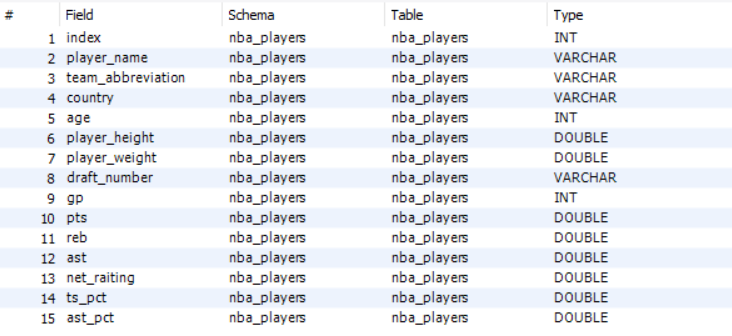
\includegraphics[width=14cm]{mysql_tables.png}
    \caption{Nazwy kolumn (atrybutów) w systemie zarządzania bazami danych MySQL}
    \label{rysunek:baza_danych}
\end{figure}

\section{Atrybuty i liczności obiektów wyrażone zmiennymi lingwistycznymi}
Definicja zmiennej lingwistycznej została już zaprezentowana w sekcji 1 we wzorze \ref{eqn_zmienna_lingwistyczna}. W aktualnej sekcji skupimy się dokładniej na tej definicji podając dla każdego z 11 atrybutów z sekcji 1 nazwę zmiennej lingwistycznej, zbiór terminów lingwistycznych oraz przestrzeń rozważań. Uważamy, że podając konkretny zbiór terminów lingwistycznych, jaki wykorzystamy, reguły gramatyczna oraz semantyczna będą widoczne i nie ma potrzeby podawania ich wprost. Wszak np. dla wzrostu nie podamy jako termin lingwistyczny słowa "zielony" lub "szybki" oraz wszystkie terminy we wszystkich zmiennych będą uporządkowane w sposób semantyczny (np. słowo "ciężki" nie wystąpi przed słowem "lekki", a słowo "idealny" przed "fatalny"). Poniżej przedstawiamy wykorzystane zmienne lingwistyczne wraz ze wzorami oraz wykresami:
\begin{enumerate}
    \item wiek zawodnika
    \begin{itemize}
        \item junior
        \begin{equation}
            \mu_{junior}(x) = \left\{\begin{matrix} 1 & dla \: x\in[18;20) \\ -0.25x + 6 & dla \: x\in [20; 24] \end{matrix}\right.
        \end{equation}
        \item młody
        \begin{equation}
            \mu_{mlody}(x) = \left\{\begin{matrix} 0.25x-5 & dla \: x\in[20;24) \\ 1 & dla \: x\in [24; 26) \\ -0.5x + 14 & dla \: x\in[26;28] \end{matrix}\right.
        \end{equation}
        \item w średnim wieku
        \begin{equation}
            \mu_{w srednim wieku}(x) = \left\{\begin{matrix} 0.5x - 13 & dla \: x\in[26;28) \\ 1 & dla \: x\in [28; 30) \\ -0.5x + 16 & dla \: x\in[30;32] \end{matrix}\right.
        \end{equation}
        \item doświadczony
        \begin{equation}
            \mu_{doswiadczony}(x) = \left\{\begin{matrix} 0.5x - 15 & dla \: x\in[30;32) \\ 1 & dla \: x\in [32; 34) \\ -0.5x + 18 & dla \: x\in[34;36] \end{matrix}\right.
        \end{equation}
        \item stary
        \begin{equation}
            \mu_{stary}(x) = \left\{\begin{matrix} 0.5x - 17 & dla \: x\in[34;36) \\ 1 & dla \: x\in [36; 44] \end{matrix}\right.
        \end{equation}
    \end{itemize}
     \begin{figure}[H]
    \centering
    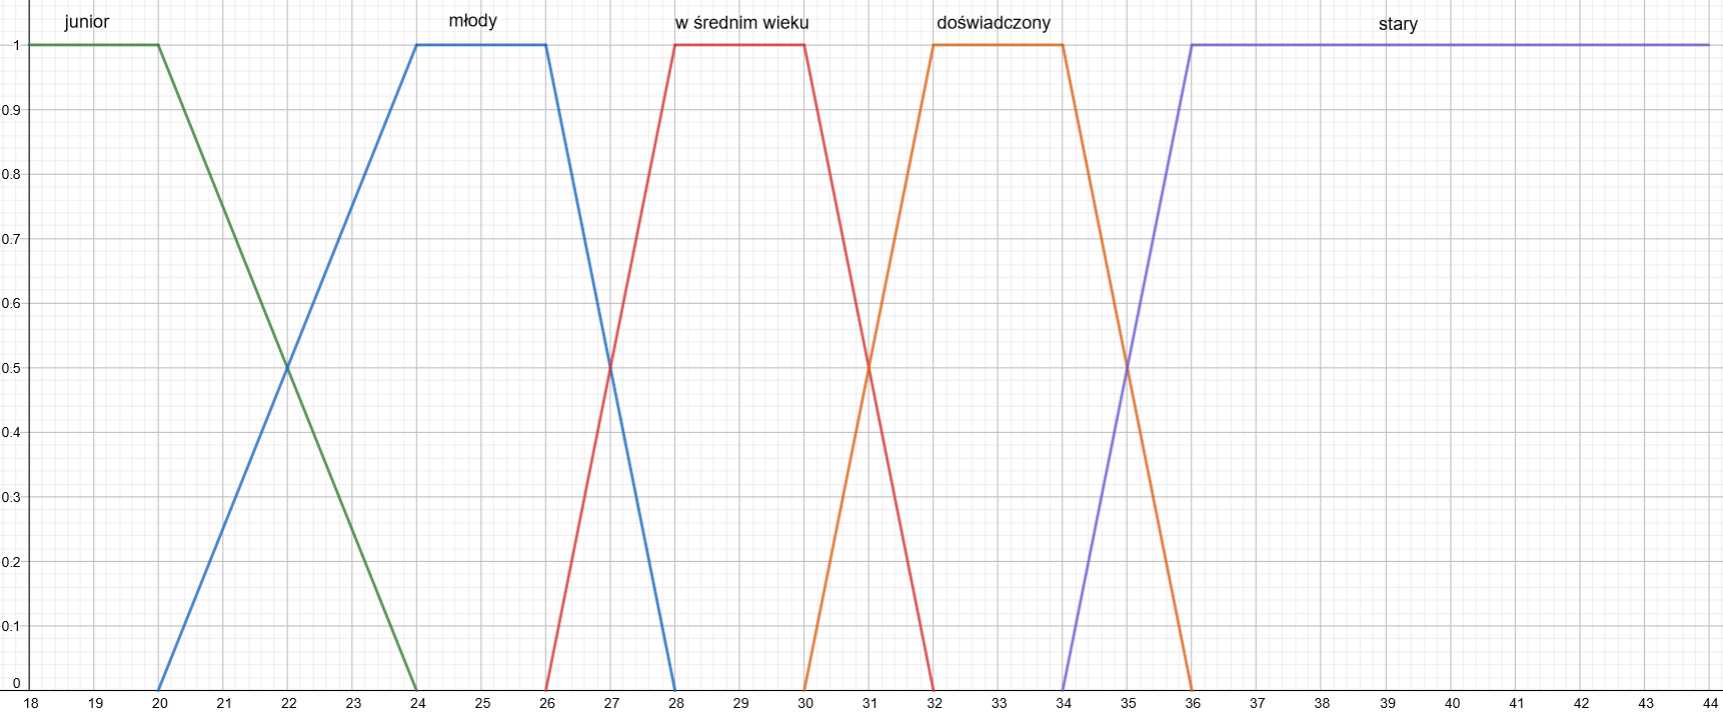
\includegraphics[width=14cm]{wykres_wiek.png}
    \caption{Wykres funkcji przynależności dla zmiennej lingwistycznej "wiek zawodnika".}
    \label{rysunek:wiek}
\end{figure}
    \item wzrost zawodnika
    \begin{itemize}
        \item niski
        \begin{equation}
            \mu_{niski}(x) = \left\{\begin{matrix} 1 & dla \: x\in[160.03;185) \\ -0.1x + 19.5 & dla \: x\in [185; 195] \end{matrix}\right.
        \end{equation}
        \item średniego wzrostu
        \begin{equation}
            \mu_{sredniegowzrostu}(x) = \left\{\begin{matrix} 0.1x - 18.5 & dla \: x\in[185;195) \\ -0.1x + 20.5 & dla \: x\in [195; 205] \end{matrix}\right.
        \end{equation}
        \item wysoki
        \begin{equation}
            \mu_{wysoki}(x) = \left\{\begin{matrix} 0.1x - 20 & dla \: x\in[200;210) \\ 1 & dla \: x\in [210; 231.14] \end{matrix}\right.
        \end{equation}
        \item bardzo niski
        \begin{equation}
            \mu_{bardzoniski}(x) = \mu_{niski}(x)^2
        \end{equation}
        \item bardzo wysoki
        \begin{equation}
            \mu_{bardzowysoki}(x) = \mu_{wysoki}(x)^2
        \end{equation}
    \end{itemize}
    Oczywiście, zgodnie z regułą semantyczną termin "bardzo niski" występuje przed terminem "niski" w zmiennej lingwistycznej. Powyżej został on wymieniony później, ponieważ definiując funkcję przynależności dla terminu "bardzo niski" korzystamy z funkcji przynależności dla terminu "niski" (konkretnie podnosimy ją do kwadratu).
    \begin{figure}[H]
        \centering
        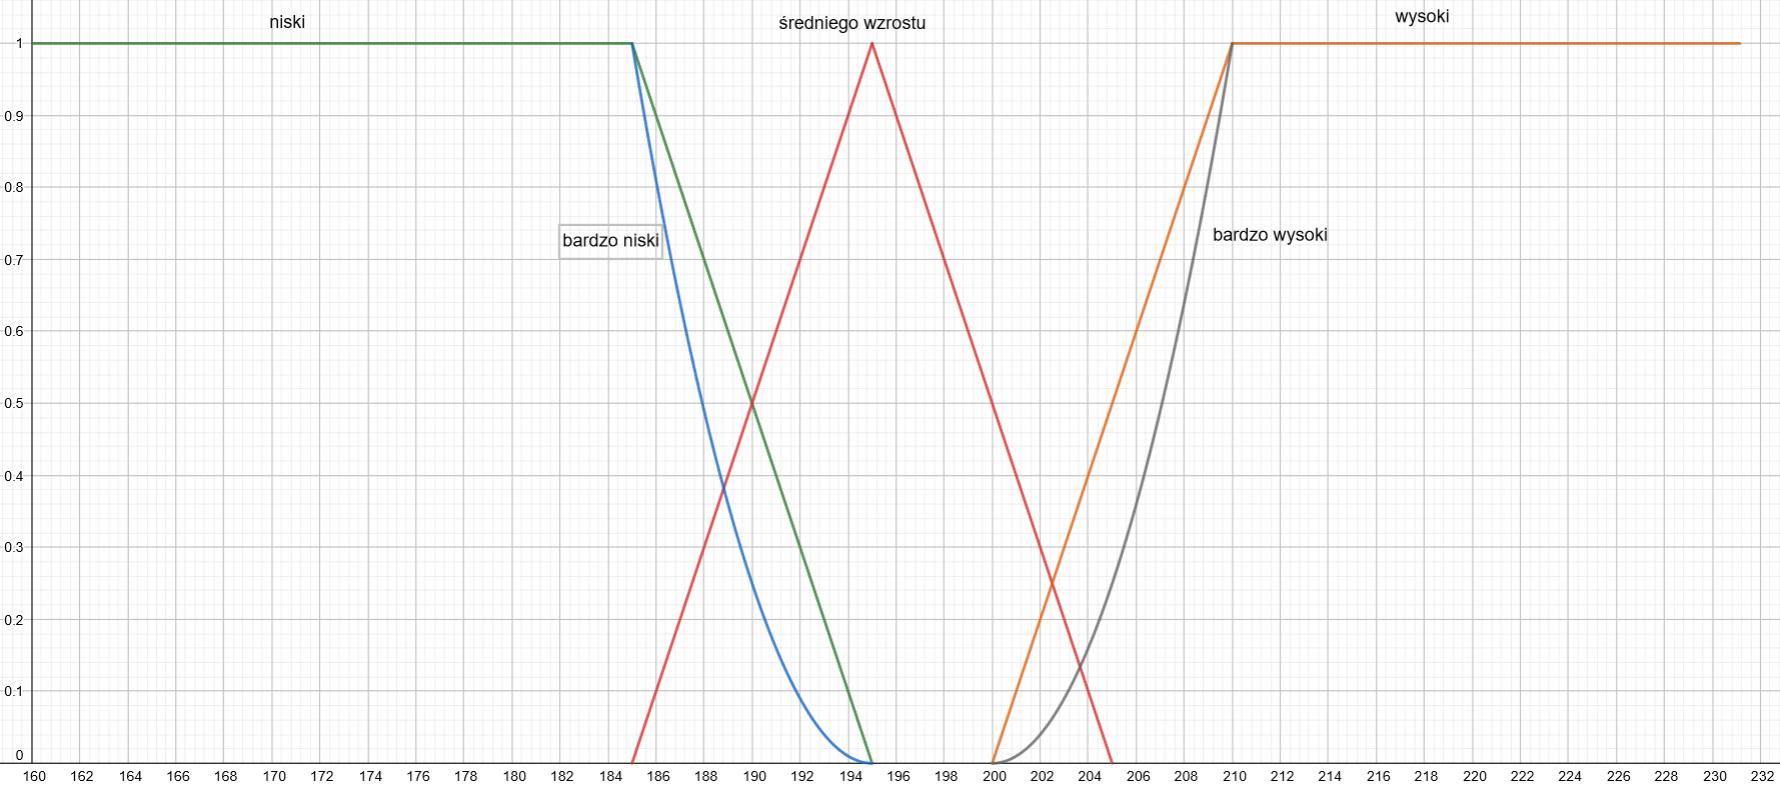
\includegraphics[width=14cm]{wykres_wzrost.png}
        \caption{Wykres funkcji przynależności dla zmiennej lingwistycznej "wzrost zawodnika".}
        \label{rysunek:wzrost}
    \end{figure}
    \item waga zawodnika
    \begin{itemize}
        \item lekki
        \begin{equation}
            \mu_{lekki}(x) = \left\{\begin{matrix} 1 & dla \: x\in[60.33;85) \\ -0.1x + 9.5 & dla \: x\in [85; 95] \end{matrix}\right.
        \end{equation}
         \item o przeciętnej wadze
        \begin{equation}
            \mu_{oprzecietnejwadze}(x) = \left\{\begin{matrix} 0.1x - 9 & dla \: x\in[90;100) \\ -0.1x + 11 & dla \: x\in [100; 110] \end{matrix}\right.
        \end{equation}
        \item ciężki
        \begin{equation}
            \mu_{ciezki}(x) = \left\{\begin{matrix} 0.1x - 10.5 & dla \: x\in[105;115) \\ 1 & dla \: x\in [115; 163.29] \end{matrix}\right.
        \end{equation}
        \item bardzo lekki
        \begin{equation}
            \mu_{bardzolekki}(x) = \mu_{lekki}(x)^2
        \end{equation}
        \item bardzo ciężki
        \begin{equation}
            \mu_{bardzociezki}(x) = \mu_{ciezki}(x)^2
        \end{equation}
    \end{itemize}
    Oczywiście, zgodnie z regułą semantyczną termin "bardzo lekki" występuje przed terminem "lekki" w zmiennej lingwistycznej. Powyżej został on wymieniony później, ponieważ definiując funkcję przynależności dla terminu "bardzo lekki" korzystamy z funkcji przynależności dla terminu "lekki" (konkretnie podnosimy ją do kwadratu).
    \begin{figure}[H]
        \centering
        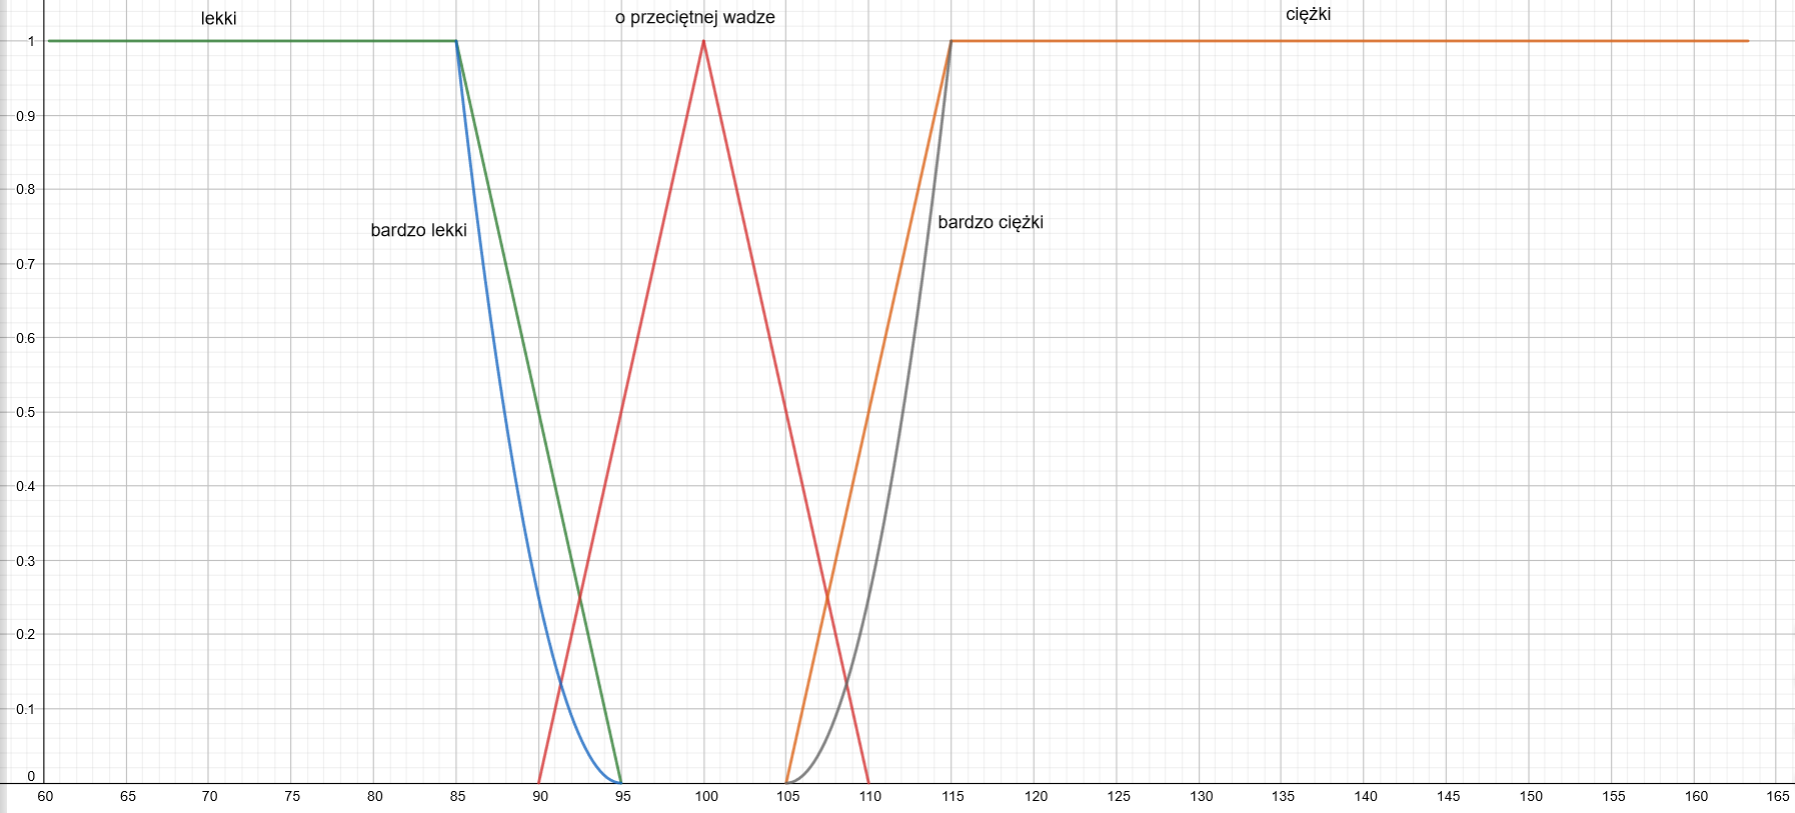
\includegraphics[width=14cm]{wykres_waga.png}
        \caption{Wykres funkcji przynależności dla zmiennej lingwistycznej "waga zawodnika".}
        \label{rysunek:waga}
    \end{figure}
\end{enumerate}

Zmienne lingwistyczne dla wybranych 10 atrybutów z bazy danych, przedstawione w
formie wykresów funkcji przynależności i wzorów analitycznych, wymienione etykiety oraz objaśnione wszystkie
symbole ułatwiające czytelnikowi ich zrozumienie \cite{zadrozny06}. Zbędne jest
cytowanie definicji. Konieczne precyzyjnie podane przestrzenie rozważań każdej
zmiennej lingwistycznej, wzory i wykresy dla każdej wartości/etykiety.\\
Jw. kwantyfikatory lingwistyczne -- opisane etykietami, wykresami funkcji
przynależności i wzorami analitycznymi. Uzasadnione wiedzą dziedzinową wybrane
zakresy i etykiety. Precyzyjnie podane przestrzenie rozważań każdego kwantyfikatora 
lingwistycznego/rozmytego, wzory i wykresy dla każdej wartości/etykiety. Opisy własne z~przypisami do literatury, tak by inżynier innej specjalności zrozumiał dalszy
opis tego konkretnego ćwiczenia/eksperymentu. \\ 
\noindent {\bf Sekcja uzupełniona jako efekt zadania Tydzień 09 wg Harmonogramu Zajęć
na WIKAMP KSR.}

\section{Narzędzia obliczeniowe: projekt (wybór, implementacja) i diagram UML pakietu obliczeń rozmytych. Diagram UML generatora podsumowań}
\subsection{Diagram pakietu obliczeń rozmytych}
Diagram UML i zwięzły opis pakietu obliczeń rozmytych: źródło pakietu
(zewnętrzny/własny/hybrydowy), przypis do literatury. Krótka charakterystyka
najważniejszych klas i podstawowych dla zadania ich metod. \\
\noindent {\bf Sekcja uzupełniona jako efekt zadania Tydzień 10 wg Harmonogramu Zajęć
na WIKAMP KSR.}

\subsection{Diagram UML generatora podsumowań. Krótka instrukcja użytkownika} 
Diagram UML generatora podsumowań (warstwy obliczeniowej oraz interfejsu
użytkownika). Krótki ilustrowany opis jak użytkownik może korzystać z aplikacji, w~szczególności
wprowadzać parametry  podsumowań, odczytywać wyniki oraz definiować własne etykiety i
kwantyfikatory. Wersja JRE i inne wymogi niezbędne do uruchomienia aplikacji przez użytkownika na własnym komputerze. \\
\noindent {\bf Sekcja uzupełniona jako efekt zadania Tydzień 11 wg Harmonogramu Zajęć
na WIKAMP KSR.}

\section{ Jednopodmiotowe podsumowania lingwistyczne. Miary jakości, podsumowanie optymalne}
Wyniki kolejnych eksperymentów wg punktów 2.-4. opisu projektu 2.  Listy podsumowań
jednopodmiotowych i tabele/rankingi podsumowań dla danych atrybutów obowiązkowe i dokładnie opisane w ,,captions'' (tytułach), konieczny opis kolumn i wierszy tabel. Dla każdego podsumowania podane miary jakości oraz miara jakości podsumowania
optymalnego.\\
\noindent {\bf Sekcja uzupełniona jako efekt zadania Tydzień 11 wg Harmonogramu Zajęć
na WIKAMP KSR.}



\section{Wielopodmiotowe podsumowania lingwistyczne i~ich miary jakości} 
Wyniki kolejnych eksperymentów wg punktów 2.-4. opisu projektu 2. Uzasadnienie i
metoda podziału zbioru danych na rozłączne podmioty. Listy podsumowań
wielopodmiotowych i tabele/rankingi podsumowań dla danych atrybutów obowiązkowe i
dokładnie opisane w ,,captions'' (tytułach), konieczny opis kolumn i wierszy tabel.
Konieczne uwzględnienie wszystkich 4-ch form podsumowań wielopodmiotowych. 
\\ 

** Możliwe sformułowanie zagadnienia wielopodmiotowego podsumowania optymalnego **.\\

{**Ewentualne wyniki realizacji punktu ,,na ocenę 5.0'' wg opisu Projektu 2. i ich porównanie do wyników z
części obowiązkowej**.}\\

\noindent {\bf Sekcja uzupełniona jako efekt zadania Tydzień 12 wg Harmonogramu Zajęć
na WIKAMP KSR.}


\section{Dyskusja, wnioski}
Dokładne interpretacje uzyskanych wyników w zależności od parametrów klasyfikacji
opisanych w punktach 3.-4 opisu Projektu 2. 
Szczególnie istotne są wnioski o charakterze uniwersalnym, istotne dla podobnych zadań. 
Omówić i wyjaśnić napotkane problemy (jeśli były). Każdy wniosek/problem powinien mieć poparcie
w przeprowadzonych eksperymentach (odwołania do konkretnych wyników: tabel i miar
jakości). Ocena które wybrane kwantyfikatory, sumaryzatory, kwalifikatory i/lub ich
miary jakości mają małe albo duże znaczenie dla wiarygodności i jakości otrzymanych
agregacji/podsumowań.  \\
\underline{Dla końcowej oceny jest to najważniejsza sekcja} sprawozdania, gdyż prezentuje poziom
zrozumienia rozwiązywanego problemu.\\

** Możliwości kontynuacji prac w obszarze logiki rozmytej i wnioskowania rozmytego, zwłaszcza w kontekście pracy inżynierskiej,
magisterskiej, naukowej, itp. **\\

\noindent {\bf Sekcja uzupełniona jako efekt zadań Tydzień 11 i Tydzień 12 wg
Harmonogramu Zajęć na WIKAMP KSR.}


\section{Braki w realizacji projektu 2.}
Wymienić wg opisu Projektu 2. wszystkie niezrealizowane obowiązkowe elementy projektu, ewentualnie
podać merytoryczne (ale nie czasowe) przyczyny tych braków. 


\begin{thebibliography}{99}
 \bibitem{niewiadomski19} A. Niewiadomski, Zbiory rozmyte typu 2. Zastosowania w reprezentowaniu informacji.  Seria „Problemy współczesnej informatyki” pod redakcją L. Rutkowskiego. Akademicka Oficyna Wydawnicza EXIT, Warszawa, 2019.
\bibitem{zadrozny06} S. Zadrożny, Zapytania nieprecyzyjne i lingwistyczne podsumowania baz danych, EXIT, 2006, Warszawa
\bibitem{niewiadomski08} A. Niewiadomski, Methods for the Linguistic Summarization of Data: Applications of Fuzzy Sets and Their Extensions, Akademicka Oficyna Wydawnicza EXIT, Warszawa, 2008.
\bibitem{nba_data} Baza danych zawierająca statystyki koszykarzy z ligi NBA z lat 1996-2020 [przeglądany 04.05.2021] Dostępna w:
https://www.kaggle.com/justinas/nba-players-data
\end{thebibliography}

Literatura zawiera wyłącznie źródła recenzowane i/lub o potwierdzonej wiarygodności,
możliwe do weryfikacji i cytowane w sprawozdaniu. 
\end{document}
